\section{Calibración geométrica mediante homogarfía}
\label{sec:homografia-tecnologias}
En muchos problemas de visión por computador, las coordenadas observadas en una imagen no representan directamente la posición real de los objetos en la escena. La perspectiva, el zoom, la posición de la cámara y los movimientos de la misma pueden hacer que dos puntos separados por la misma distancia física aparezcan a distancias muy distintas en píxeles. Por este motivo, cuando se desea razonar sobre posiciones reales, resulta necesario calibrar la cámara y transformar puntos desde el plano de la imagen hacia un plano de referencia.

\subsection{Homografía entre planos}

Cuando la superficie observada puede aproximarse como un plano, la relación entre los puntos de la imagen y los puntos de dicho plano puede modelarse mediante una homografía. Una homografía es una transformación proyectiva \footnote{Una transformación proyectiva es una operación geométrica que mapea puntos de un plano (o espacio) a otro, preservando las líneas rectas pero no necesariamente el paralelismo, ángulos o distancias} entre dos planos, representada mediante una matriz $H \in \mathbb{R}^{3 \times 3}$. En este contexto, permite relacionar coordenadas en píxeles de la imagen broadcast con coordenadas sobre una representación 2D del terreno de juego.

Para expresar esta transformación se utilizan coordenadas homogéneas. Este tipo de representación consiste en añadir a un punto bidimensional como $(u,v)$, una tercera componente y se escribe como $(u,v,1)$. Esta representación permite describir transformaciones de perspectiva mediante una multiplicación matricial. Así, un punto de imagen $(u,v)$ y su correspondiente punto del plano de referencia $(x,y)$ se relacionan mediante:

\[
\begin{bmatrix}
x \\
y \\
1
\end{bmatrix}
\sim
H
\begin{bmatrix}
u \\
v \\
1
\end{bmatrix}
\]

Tras aplicar la matriz, las coordenadas resultantes se normalizan dividiendo por la tercera componente para volver a obtener coordenadas bidimensionales.

La \hyperref[fig:exp-homografia]{Figura~\ref*{fig:exp-homografia}} muestra una interpretación geométrica de esta idea, en la que los puntos de un plano se proyectan sobre otro plano, estableciendo una correspondencia entre ambas superficies.

\begin{figure}[H]
    \centering
    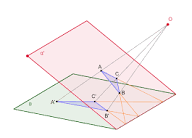
\includegraphics[width=0.3\textwidth]{Imagenes/Propias/exp_homografia.png}
    \caption[Esquema de homografía entre planos]{
Esquema geométrico de una homografía entre dos planos proyectivos. Los puntos del plano original se proyectan desde un centro de proyección sobre un segundo plano, estableciendo una correspondencia entre ambas superficies. Fuente: reproducida de \citep{DibujoSecundariaTransformaciones}.
}
    \label{fig:exp-homografia}
\end{figure}

Esta transformación no conserva necesariamente distancias, ángulos ni áreas, pero sí permite transformar puntos entre dos planos cuando existen suficientes correspondencias geométricas. Estas correspondencias pueden obtenerse a partir de elementos conocidos de la escena. Si se identifican suficientes referencias, es posible estimar la homogradia que alinea la imagen con una representación métrica del plano observado.

\subsection{Estimación de homografía mediante PnLCalib}
PnLCalib \citep{GutierrezPnLCalib2024} es un método de calibración de cámaras en vídeo deportivo diseñado para obetener una transformación geométrica que permita proyectar la imagen broadcast sobre un modelo geométrico del campo de fútbol. A diferencia de otros enfoques que dependen únicamente de puntos característicos o de una búsqueda sobre posibles poses de cámara, PnLCalib combina información de puntos y líneas del terreno de juego para obtener una estimación más robusta.

El método parte de una idea sencilla: el campo de fútbol tiene una geometría conocida. Líneas de banda, áreas, círculo central, puntos de penalti e intersecciones entre marcas del terreno pueden utilizarse como referencias para estimar la relación entre la imagen y el modelo del campo. Para ello, PnLCalib emplea redes encoder-decoder que predicen mapas de calor de \textit{keypoints} y extremos de líneas visibles en el frame. A partir de estas predicciones se extraen correspondencias entre la imagen y el modelo geométrico del campo.

El proceso general de PnLCalib se resume en la \hyperref[fig:pnlcalib-pipeline]{Figura~\ref*{fig:pnlcalib-pipeline}} y se divide en dos etapas principales: la generación de datos de entrenamiento y la fase de inferencia.

En la primera etapa, el método parte de las anotaciones de SoccerNet y de la geometría conocida del campo de fútbol para construir las referencias que aprenderán las redes. El resultado de esta etapa no es un nuevo conjunto de imágenes, sino un conjunto de pares de entrenamiento en los que cada frame queda asociado a 57 mapas de calor que indican la posición esperada de 57 puntos característicos del terreno de juego y a 23 mapas de calor de las líneas del campo.

Durante la fase de inferencia, PnLCalib recibe un frame de entrada y utiliza dos redes encoder-decoder. La primera red predice $57+1$ mapas de calor: un canal para cada \textit{keypoint} predefinido y un canal adicional de fondo. Cada mapa de calor indica la probabilidad de que el punto correspondiente se encuentre en cada posición de la imagen, por lo que la localización final del punto se obtiene seleccionando las zonas de mayor activación. La segunda red predice $23+1$ mapas de calor asociados a las líneas del campo: un canal por cada línea considerada y un canal adicional de borde. En este caso, cada canal contiene dos activaciones principales, correspondientes a los extremos visibles de la línea.

A partir de los máximos de estos mapas de calor se extraen las posiciones en la imagen de los puntos característicos y de los extremos de las líneas en la imagen. Además, las líneas detectadas pueden utilizarse para recuperar puntos no observados directamente mediante intersecciones entre líneas, aumentando así el número de referencias disponibles. Además las posiciones en el modelo del campo de todas esas referencias son conocidas, por tanto, con estas correspondencias entre la imagen y el modelo geométrico del campo se calcula una calibración inicial mediante métodos geométricos.

Finalmente, PnLCalib incorpora un módulo de refinamiento PnL, de \textit{Points and Lines}, que ajusta la calibración inicial utilizando conjuntamente la información de puntos y líneas. Este refinamiento se plantea como un problema de optimización no lineal orientado a reducir el error de reproyección, es decir, la diferencia entre las referencias observadas en la imagen y las referencias proyectadas desde el modelo geométrico del campo.

\begin{figure}[H]
    \centering
    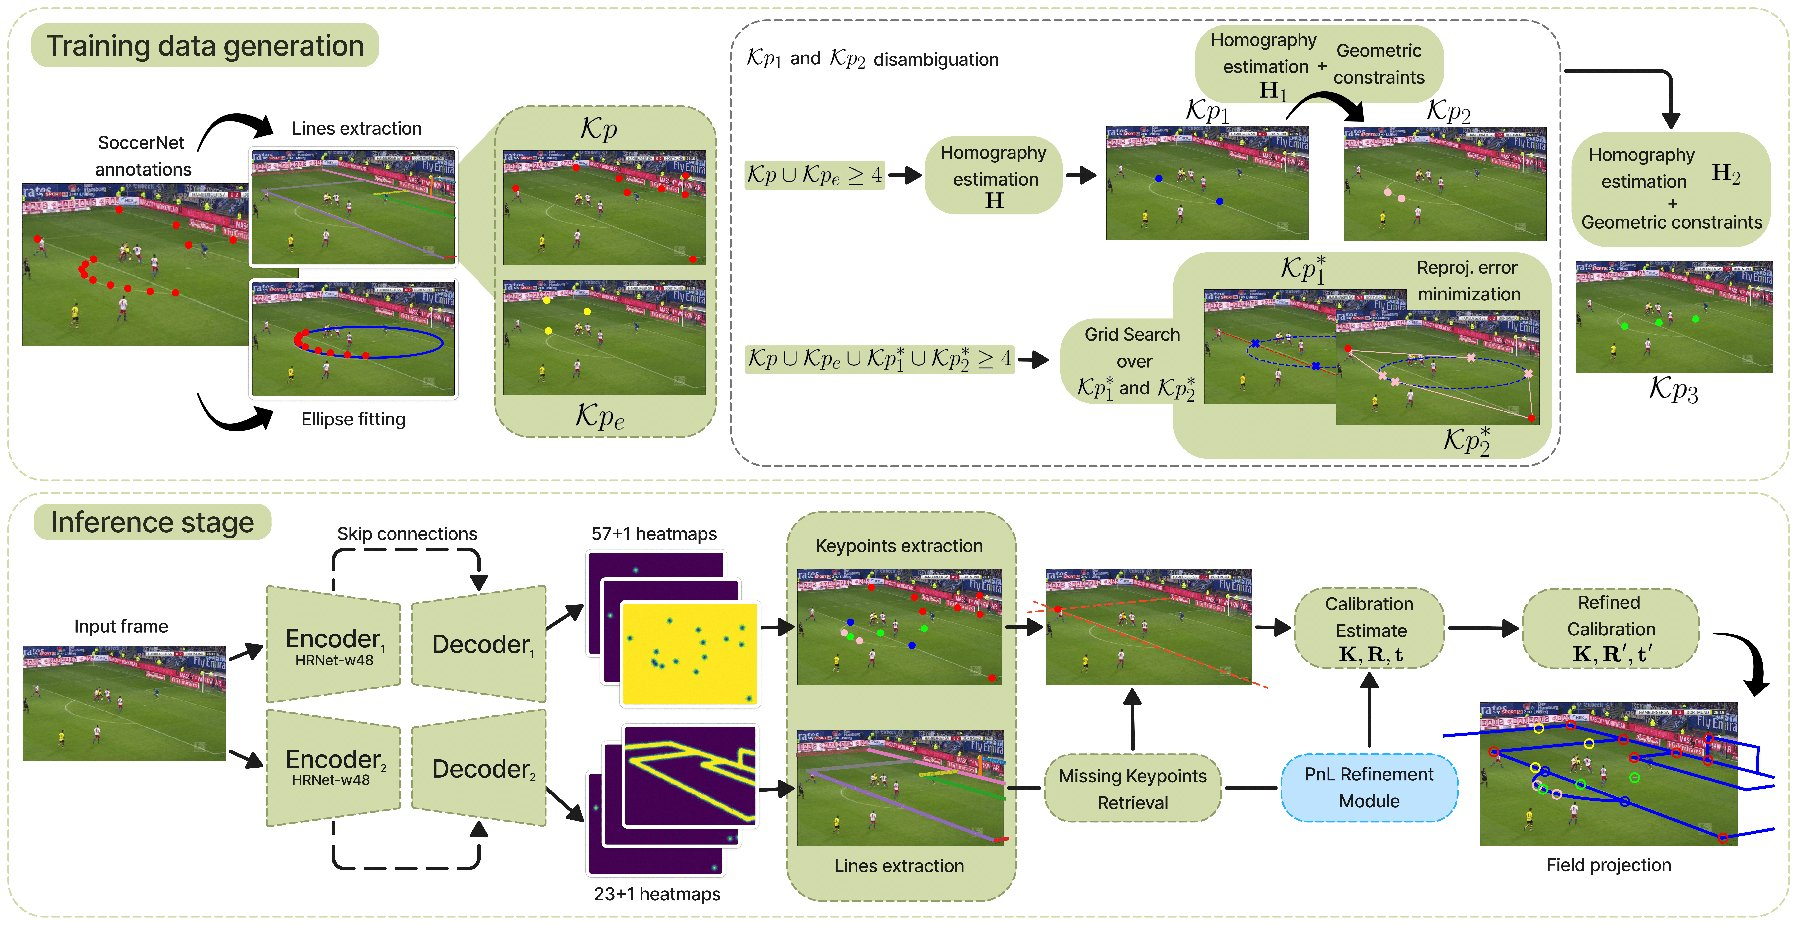
\includegraphics[width=0.9\textwidth]{Imagenes/Propias/pipeline.jpg}
    \caption[Pipeline de PnLCalib]{
    Pipeline de PnLCalib para estimar la calibración del campo mediante \textit{keypoints}, líneas y refinamiento geométrico. Fuente: reproducida de \citep{GutierrezPnLCalib2024}.
    }
    \label{fig:pnlcalib-pipeline}
\end{figure}

La \hyperref[fig:field-reconstruction]{Figura~\ref*{fig:field-reconstruction}} muestra un ejemplo visual de este proceso. Las líneas proyectadas representan la estructura geométrica estimada del campo sobre la imagen original, mientras que los puntos coloreados indican referencias detectadas o utilizadas durante el ajuste. Este tipo de visualización permite comprobar de forma intuitiva si la calibración obtenida es coherente con la escena observada.

\begin{figure}[H]
    \centering
    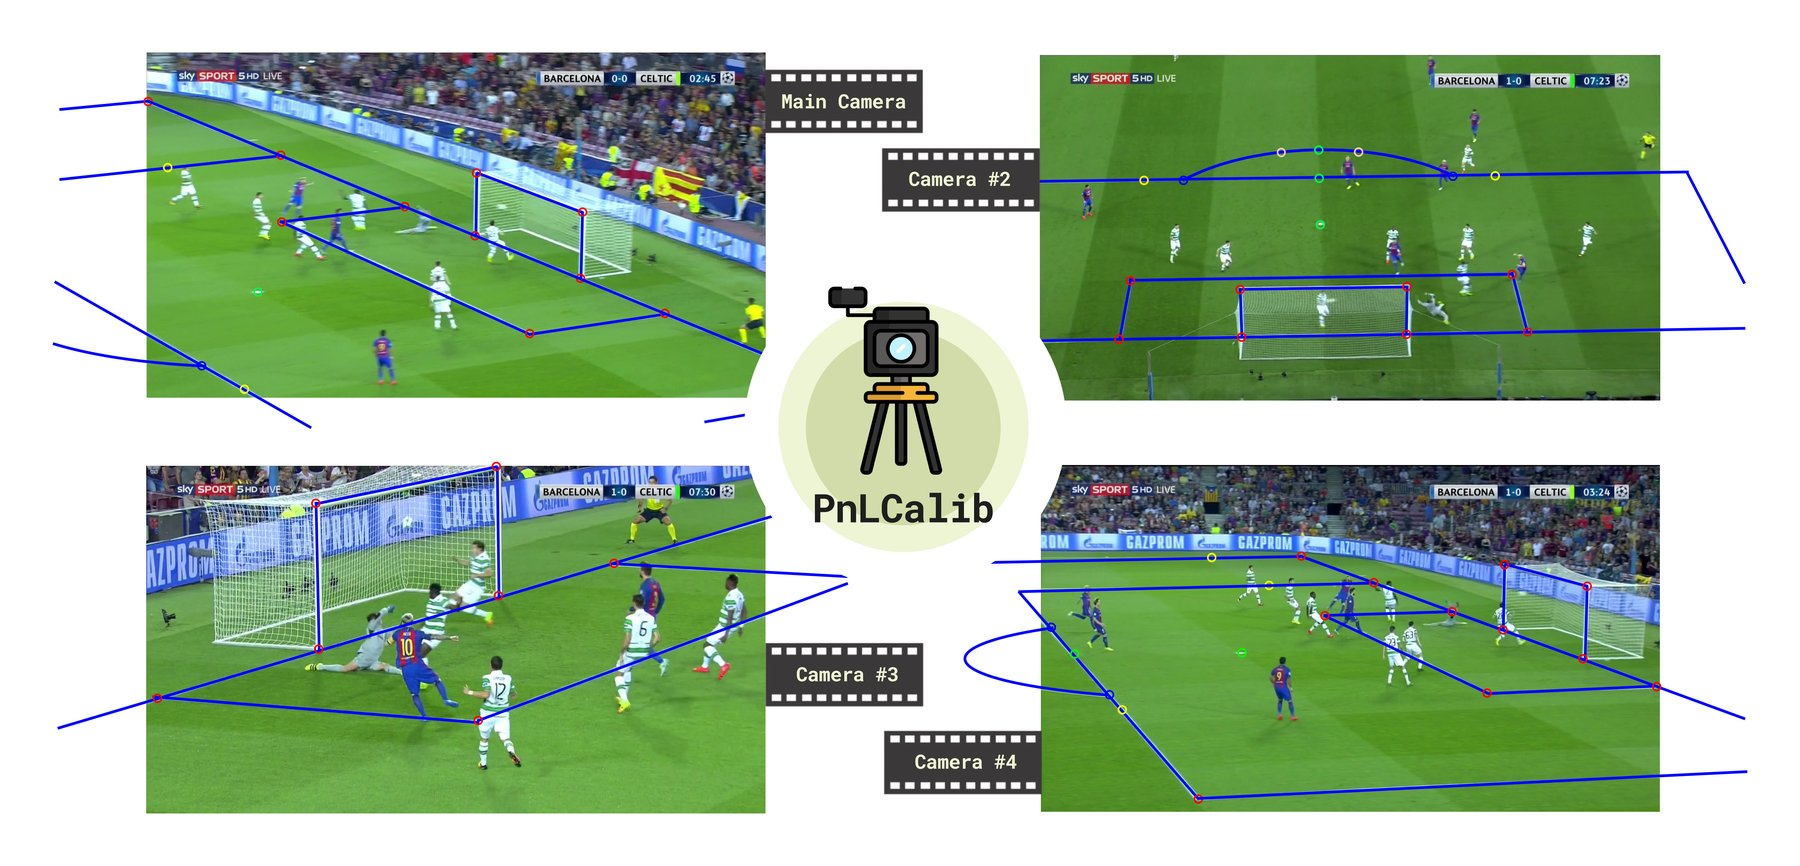
\includegraphics[width=0.95\textwidth]{Imagenes/Propias/field_reconstruction.jpg}
    \caption[Reconstrucción geométrica sobre imágenes broadcast]{
    Reconstrucción geométrica sobre imágenes broadcast mediante líneas y puntos de referencia. Fuente: reproducida de \citep{PnLCalibRepo2024}.
    }
    \label{fig:field-reconstruction}
\end{figure}

\subsection{Papel de la homografía dentro del pipeline}
En el contexto de este proyecto, la homografía permite transformar las detecciones obtenidas en la imagen broadcast hacia una representación 2D del terreno de juego. De esta forma, las detecciones obtenidas en píxeles pueden expresarse en un sistema de coordenadas más próximo al espacio físico real del partido.

Una vez estimada la homografía, cada detección puede proyectarse al campo a partir de un punto representativo. En el caso de los jugadores, se utiliza habitualmente el punto inferior central de la \textit{bounding box}, ya que aproxima la posición de contacto del jugador con el plano del suelo.

La principal ventaja de trabajar en coordenadas del campo es que las distancias pasan a tener una interpretación física. Esto resulta útil para etapas posteriores del pipeline, como el tracking multiobjeto, la clasificación posicional o el análisis de eventos. Por ejemplo, una identidad perdida puede recuperarse si reaparece en una posición compatible sobre el terreno de juego.

No obstante, la calibración también introduce riesgos. Si la homografía estimada es incorrecta, todas las posiciones proyectadas quedarán desplazadas de forma sistemática. En vídeo broadcast, este problema puede aparecer cuando la cámara cambia bruscamente, cuando se observa una zona reducida del campo o cuando las líneas visibles son insuficientes. Por este motivo, la homografía debe tratarse como una señal valiosa, pero no infalible, y conviene que el pipeline pueda continuar aunque algunos frames no dispongan de una proyección fiable.

La integración concreta de la calibración en el sistema desarrollado, incluyendo las estrategias de robustez y los criterios prácticos de aceptación de homografías, se describe posteriormente en la 
\hyperref[sec:calibracion-campo-proyeccion-metricas]{Sección~\ref*{sec:calibracion-campo-proyeccion-metricas}}
